\chapter{Campagna sperimentale}

\section{Approccio}

\subsection{10-folds cross validation}
Per la fase di training dei modelli viene utilizzata la tecnica k-folds cross validation. Si procede quindi creando una partizione del dataset iniziale, dove ogni sottoinsieme, ovvero un fold, ha circa lo stesso numero di istanze ed è più o meno bilanciato tra la classe positiva e negativa.

Per gli esperimenti effettuati, è stato scelto $k = 10$, ovvero il dataset viene diviso casualemnte in 10 parti, utilizzando ad ogni iterazioni una porzione di dati diversa per il trainig-set e test-set. Avendo scelto questo valore di k, la proporzione tra i due insiemi sarà sempre 90\% per il training-set e 10\% per il test-set.

Per ogni modello si vogliono testare diversi iperparametri (\autoref{sec:mode_selection}), pertanto ad ogni iterazione della 10-folds, fissato un fold per il training $\hat{F}$, si esegue un'altra 10-fold cross validation più interna su $\hat{F}$  ($90\%$ del dataset totale), così da poter scegliere l'iperparametro migliore.

Procedendo in questo modo l'ottimizzazione degli iperparametri viene effettuata sfruttando solo il training set e il test set non viene utilizzato nè per il training nè per la scelta degli iperparametri ottimali.

\begin{figure}[H]
	\centering
	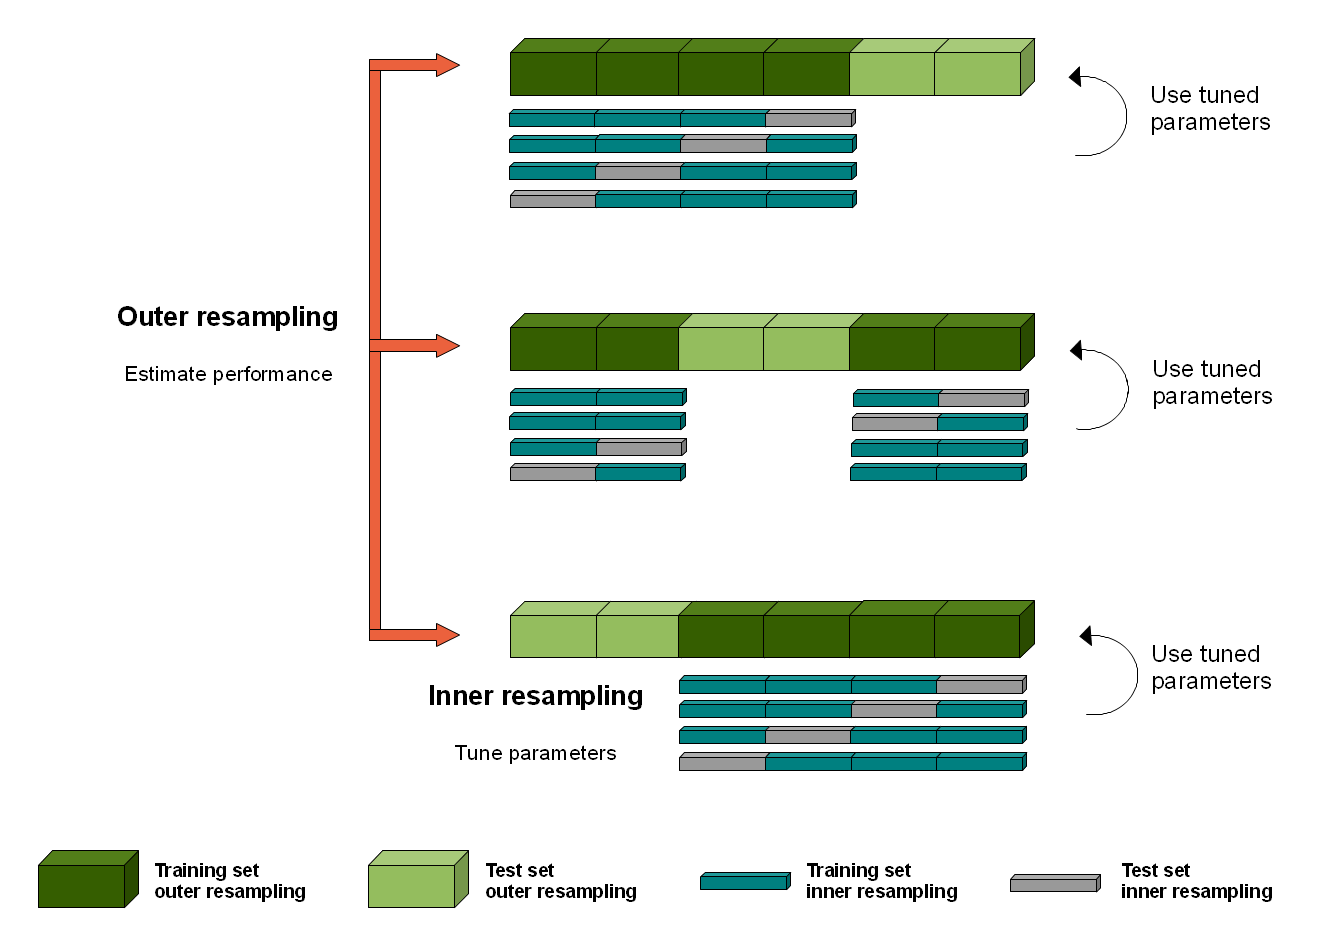
\includegraphics[width=13cm]{assets/nested-cv.png}
	\caption{Nested 3-folds cross validation.}
\end{figure}

Una nota importante è che i 10 folds vengono generati in modo casuale, tuttavia per ogni modello di cui si vuole fare il training, questa generazione casuale viene effettuata a per mezzo dello stesso seed. Questo garatisce di avere folds generati casualmente ma in modo idenctico per ogni modello, in questo modo si ottengono dei risultati statisticamente validi.

\subsection{Model selection}
\label{sec:mode_selection}
Come abbiamo sopra discusso, per ogni modello viene effettuato il tuning degli iperparametri usando la tecnica 10-folds cross validation.

\subsubsection{Grid search}
\label{sec:grid-search}
Per determinare gli iperparametri ottimali, vengono scelti un insieme di parametri da utilizzare per la fase di training dei modelli. Per ogni modello si considerando tutte le combinazioni dei valori scelti per i parametri.


TODO: I parametri di cp non sono veri.
\begin{table}[H]
	
	\begin{center}
		
		\begin{tabular}{| l | l | l | l |}
			\hline
			\multicolumn{2}{|c|}{\textbf{SVM -  RBF kernel}} &
			\multicolumn{1}{|c|}{\textbf{SVM - Linear kernel}} &
			\multicolumn{1}{c|}{\textbf{Decision tree}}\\
			\hline
			\hline
			\multicolumn{1}{|c}{$C$} &
			\multicolumn{1}{c|}{$sigma$} &
			\multicolumn{1}{c|}{$C$ } &
			\multicolumn{1}{c|}{$cp$}\\
			\hline
			0.001	 & 0.00001    & 0.000001 & \textbf{0.01580381}\\
			0.01	  & 0.0001      &0.00001	& 0.03487738\\
			0.1	   & 0.001      	&0.0001	   & 0.17983651\\
			\textbf{1}			& 0.01      	  &0.001		  & \\
			10	   &\textbf{ 0.1 }     	  &0.01		   & \\
			&       		   	     &\textbf{0.1}			   & \\
			&       	  			 &1				& \\
			&       	  			 &10			   & \\
				  		   
			\hline
		\end{tabular}
		
	\end{center}
	\caption{Tabella iperparametri utilizzati per grid search.}
\end{table}

I valori in grassetto nella tabella sono gli iperparametri ottimali.
Per quanto riguarda il parametro complexity parameter di decision tree, l'insieme dei valori non è stato scelto manualmente.


\section{Misure di performance}
Le misure di performance sono state ottenute combinando i risultati
ottenuti dalla 10-fold cross validation per ogni fold sia per la
classe positiva che per la classe negativa facendo la macro average
delle misure cercate.

\subsection{Accuracy}
L'accuracy é definita come il numero di veri positivi e veri negativi
rapportati al numero di esempi totali.

Per i modelli esaminati abbiamo ottenuto:

\subsection{Precision}
La precision é definita come il numero di veri positivi rapportati al
numero totale di predizioni positive.

Per i modelli esaminati abbiamo ottenuto:
\subsection{Recall}
La misura di recall é definita come il numero di veri positivi
rapportati al numero di veri positivi e falsi negativi.

Per i modelli esaminati abbiamo ottenuto:
\subsection{F-measure}
La F-Measure é definita come la media armonica di precision e
sensitivity.

Per i modelli esaminati abbiamo ottenuto:
\subsection{Curve ROC e AUC}

\section{Support Vector Machine}
\subsection{Kernel}

\section{Decision Tree} \subsection{Scelta del modello} Come secondo
modello parte del progetto é stato scelto un albero di decisione
(decision tree/classification tree). Questo perché anche con un
dataset relativamente ampio permette il training in un tempo
ragionevole rispetto alla potenza computazionale in nostro possesso.

\subsection{Complexity Parameter}
\subsection{Decision Tree Plot}
\subsection{Risultati esperimenti}
\subsubsection{Performance classe positiva vs negativa}
\begin{figure}[H]
	  \subfloat[SVM - RBF.]{
	\begin{minipage}[c]{0.5\textwidth}
		\centering
		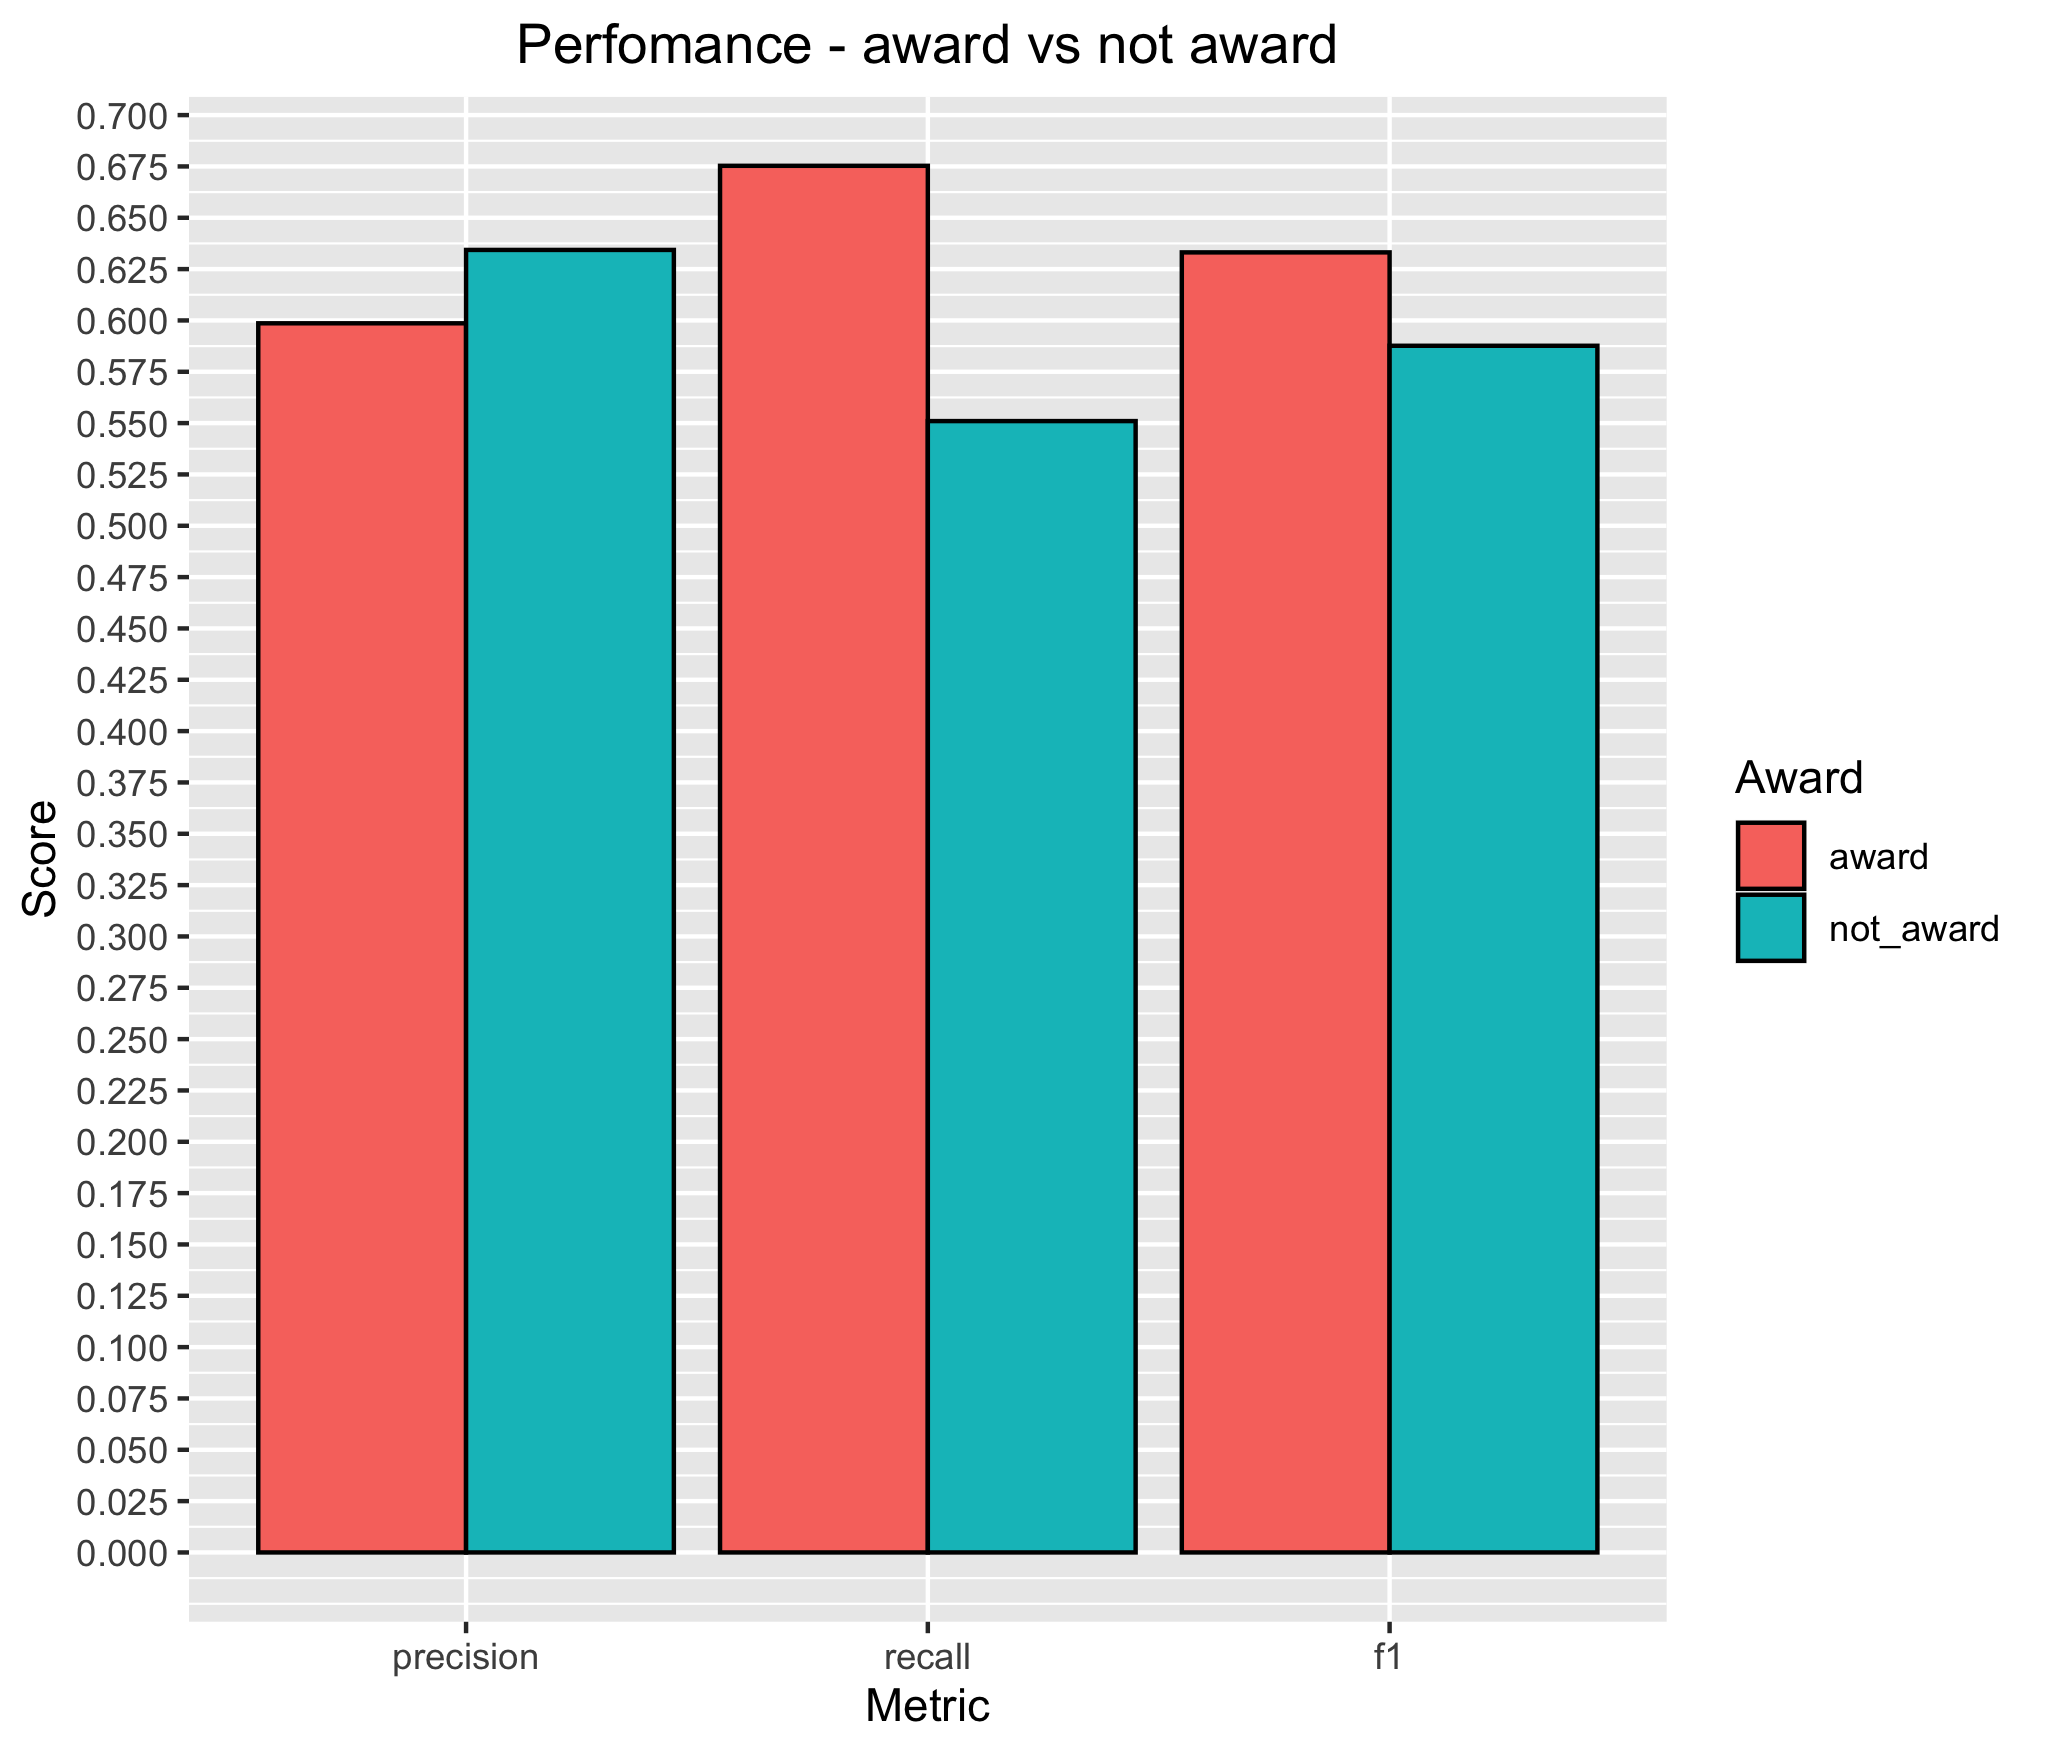
\includegraphics[width=7cm]{../images/svmRadial_class_performance.png}
\end{minipage}}
\hfill 	
\subfloat[SVM - Linear.]{
	\begin{minipage}[c]{0.5\textwidth}
		\centering
		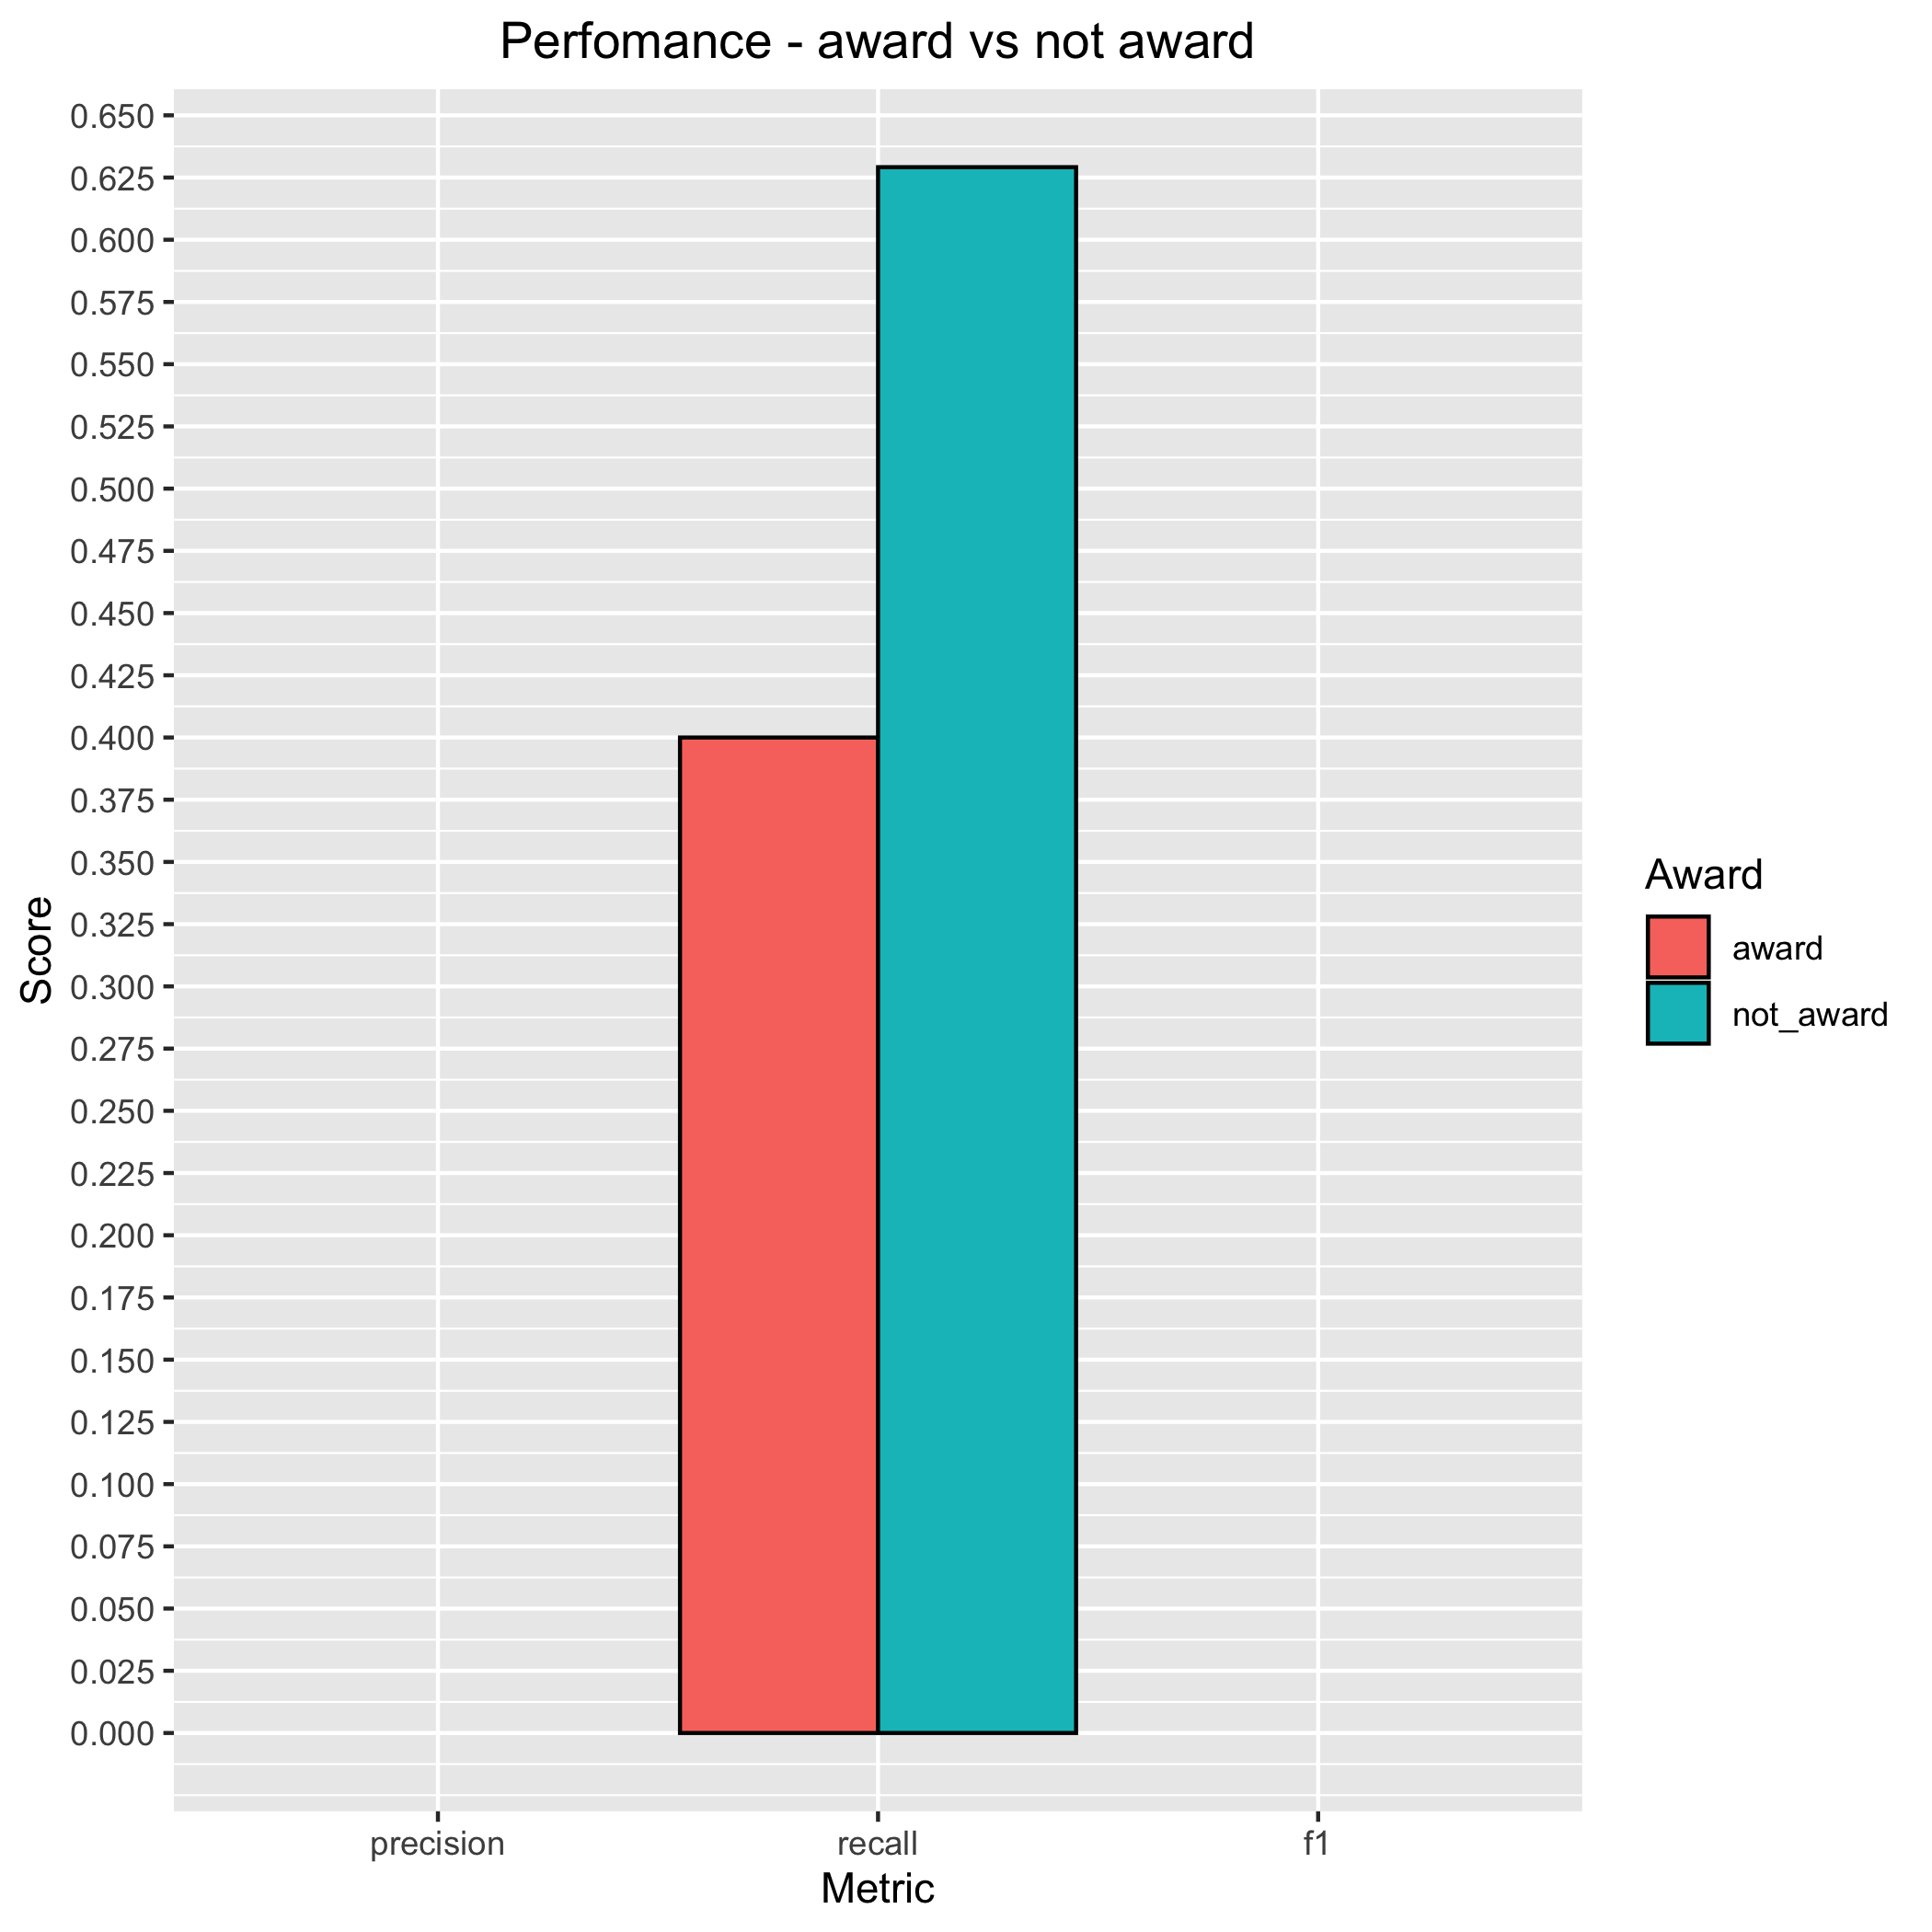
\includegraphics[width=7cm]{../images/svmLinear_class_performance.png}
\end{minipage}}

\subfloat[Decision tree.]{
	\begin{minipage}[c]{\textwidth}
		\centering
		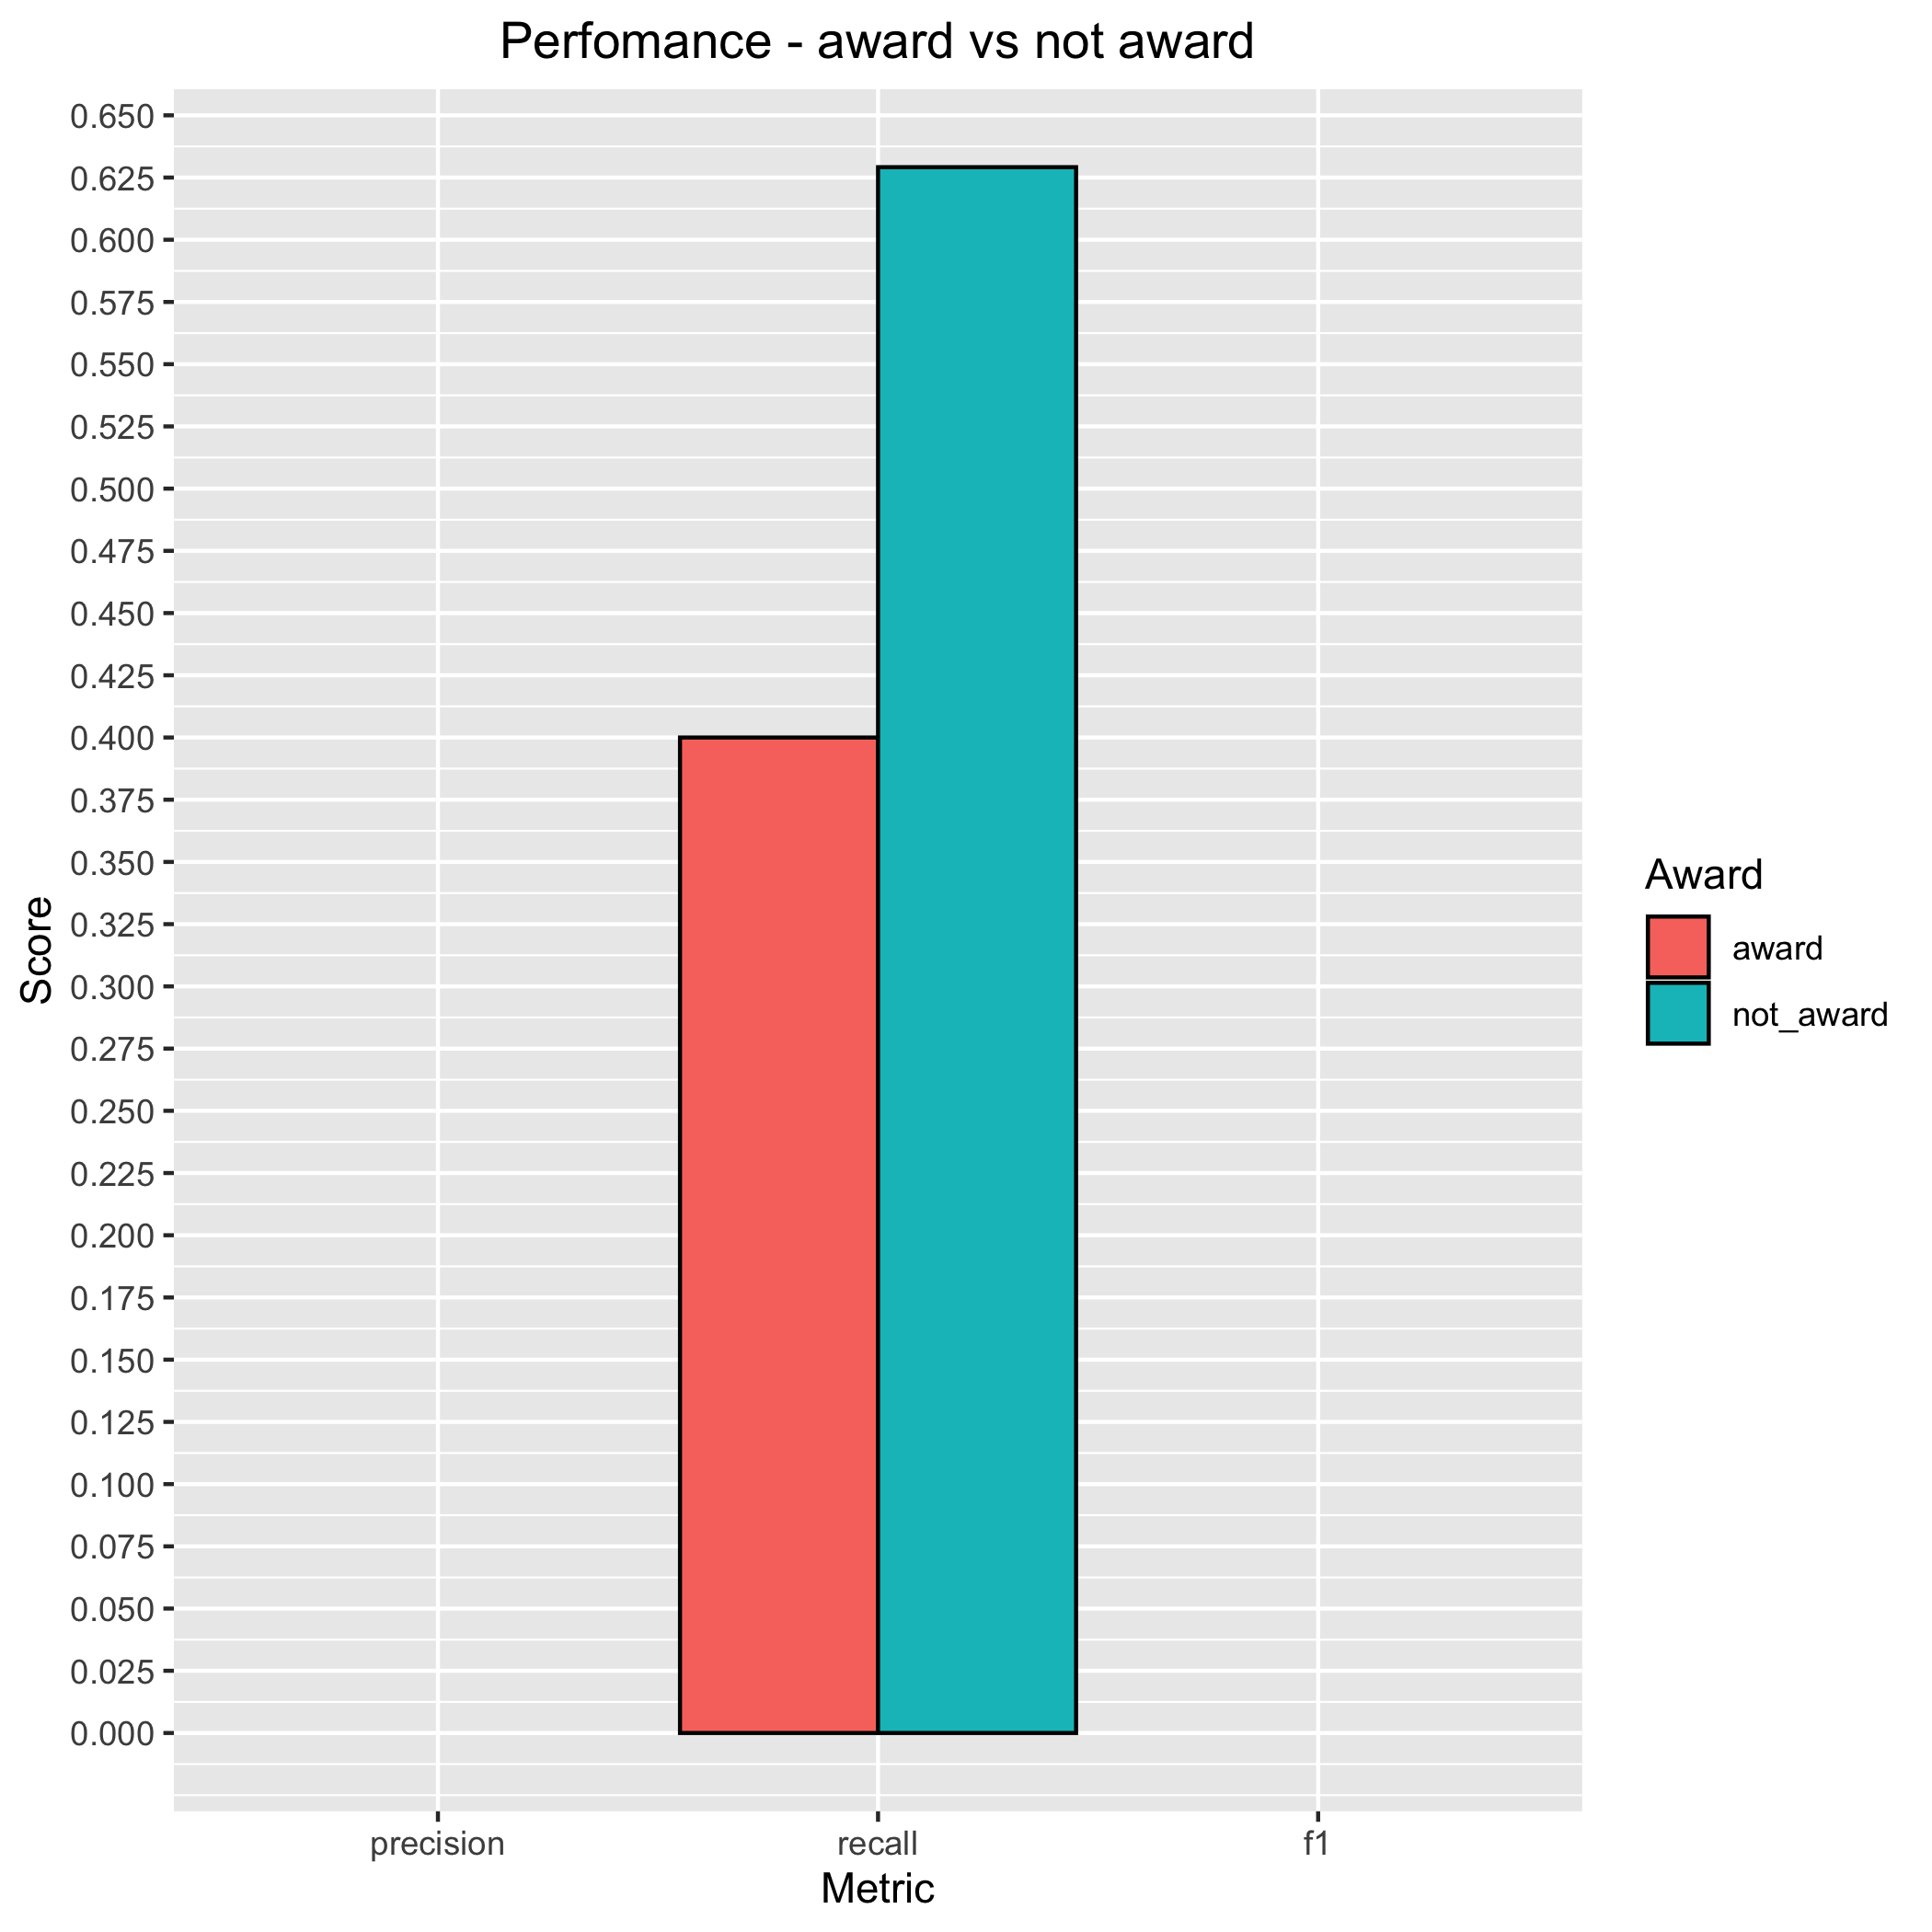
\includegraphics[width=7cm]{../images/svmLinear_class_performance.png}
\end{minipage}}

\caption{Performance dei modelli distinguendo tra classe positiva e negativa.}
\end{figure}

\subsubsection{Performance macro average}
\begin{figure}[H]
	\centering
	\begin{subfigure}[b]{0.3\textwidth}
		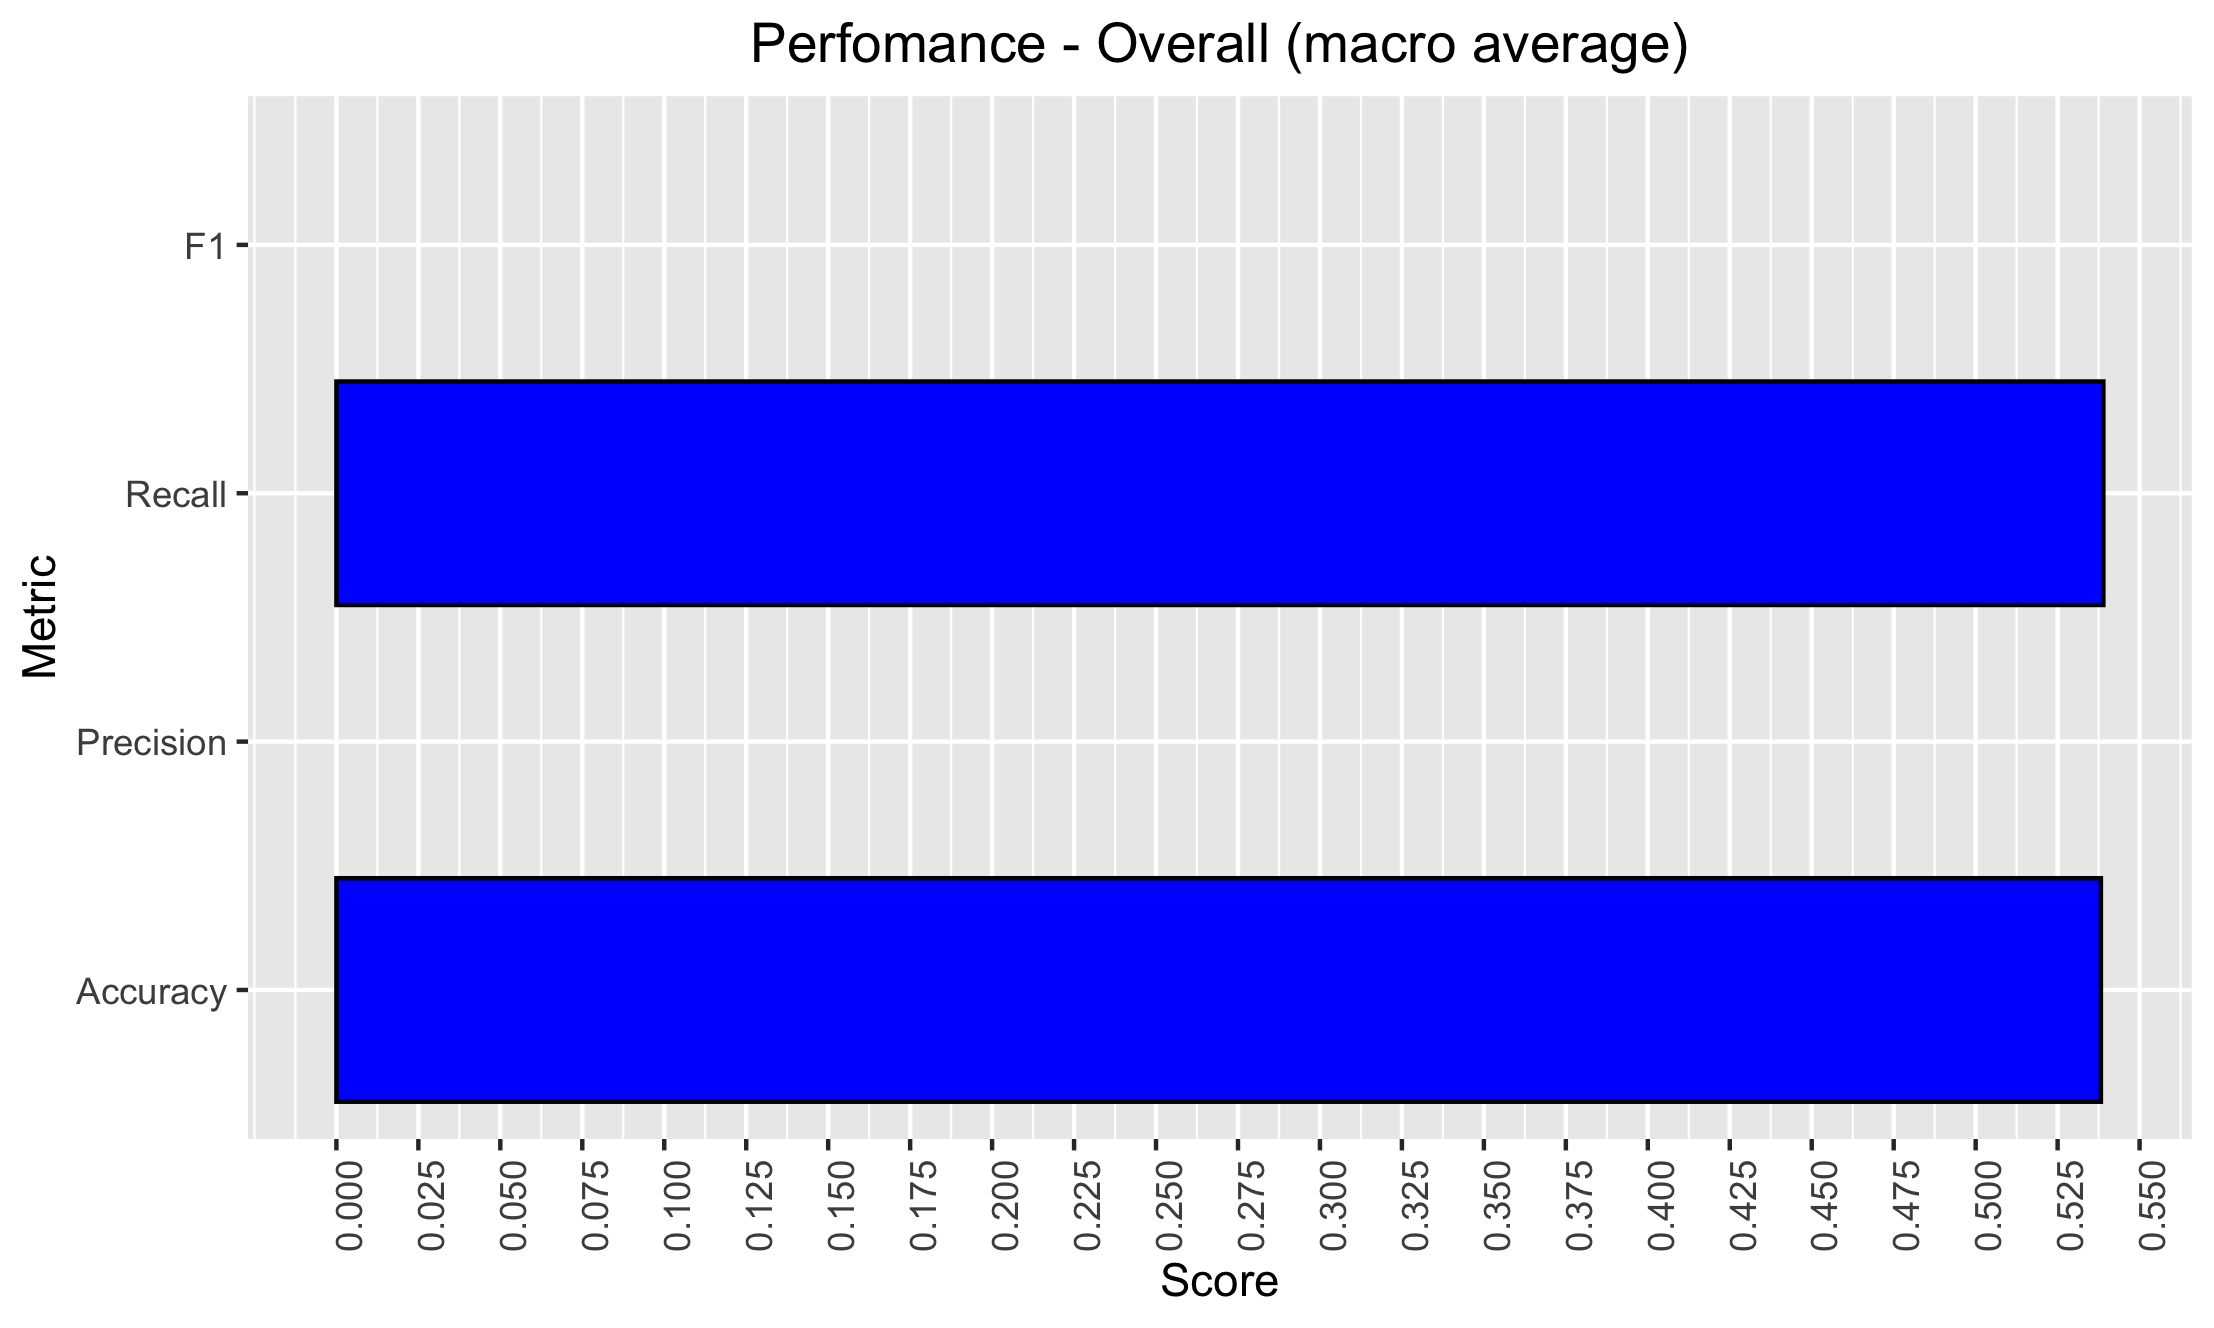
\includegraphics[width=4.25cm]{../images/svmRadial_performance.png}
		\caption{SVM - RBF.}
	\end{subfigure}
	\begin{subfigure}[b]{0.3\textwidth}
		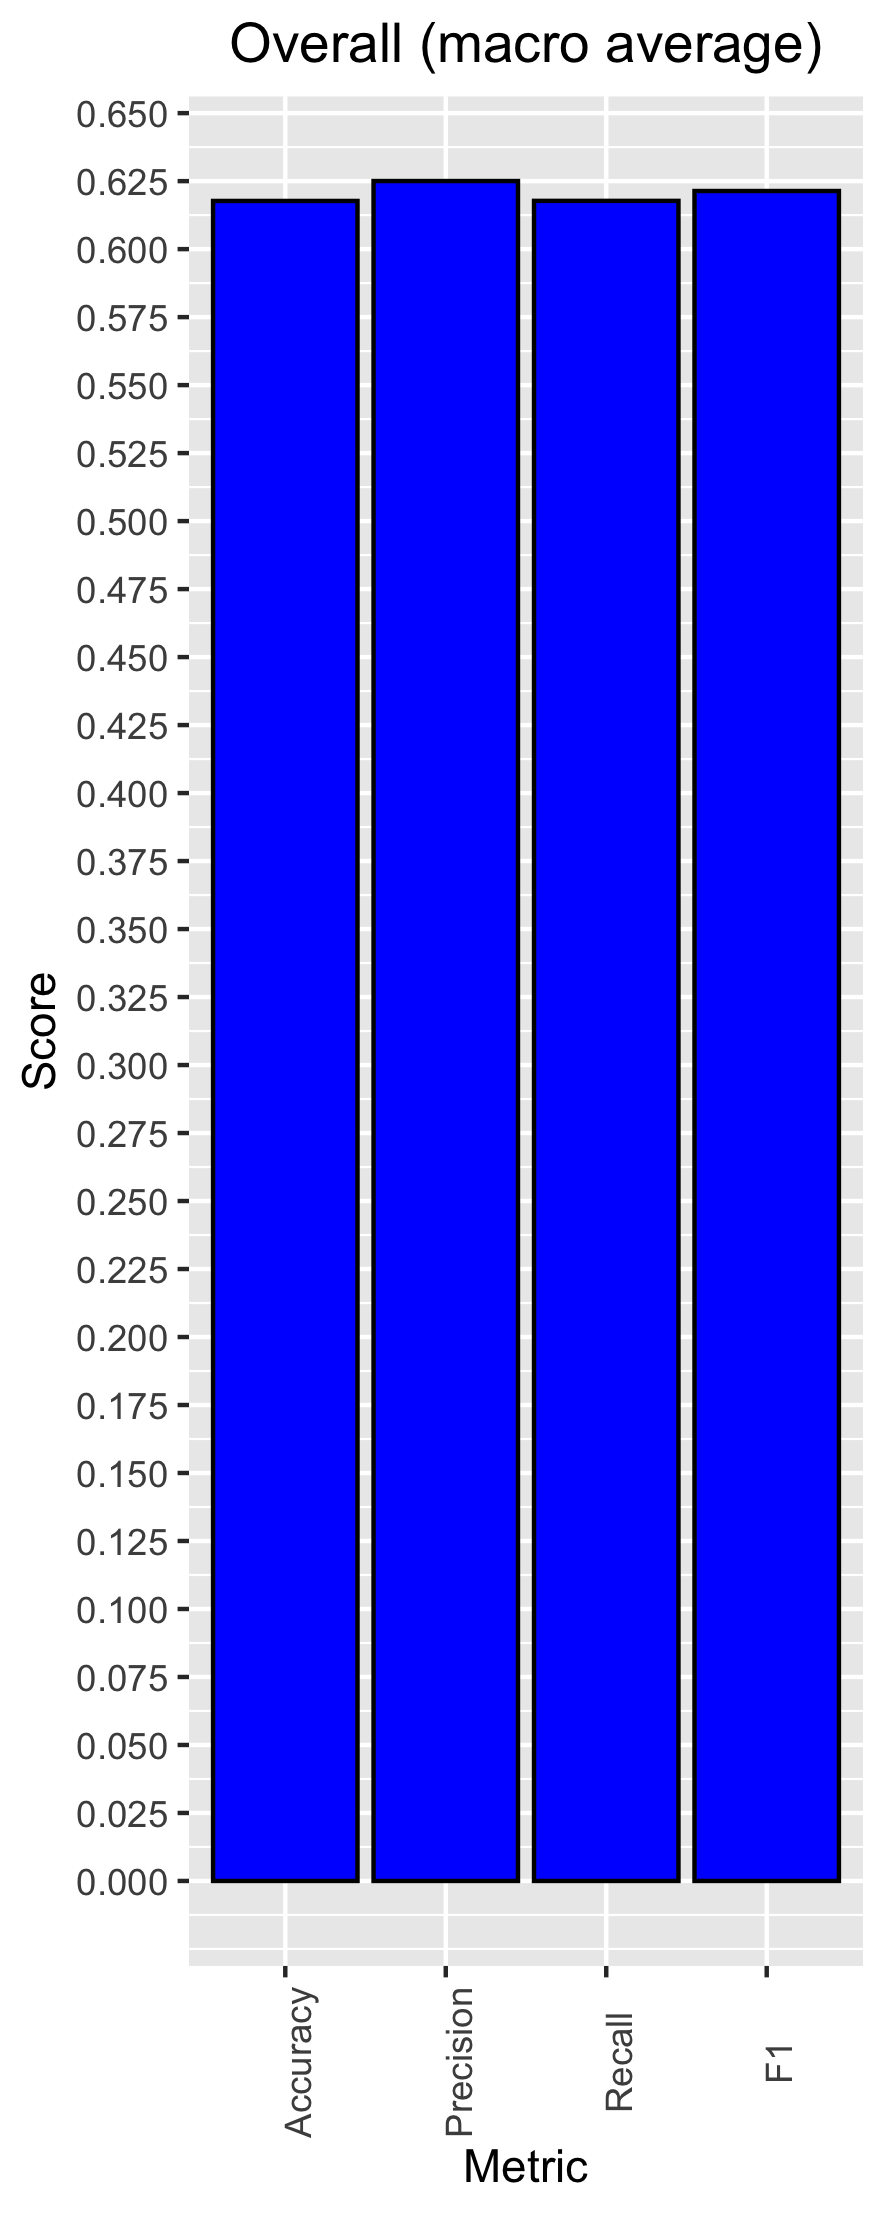
\includegraphics[width=4.25cm]{../images/svmLinear_performance.png}
		\caption{SVM - Linear.}
	\end{subfigure}
	\begin{subfigure}[b]{0.3\textwidth}
		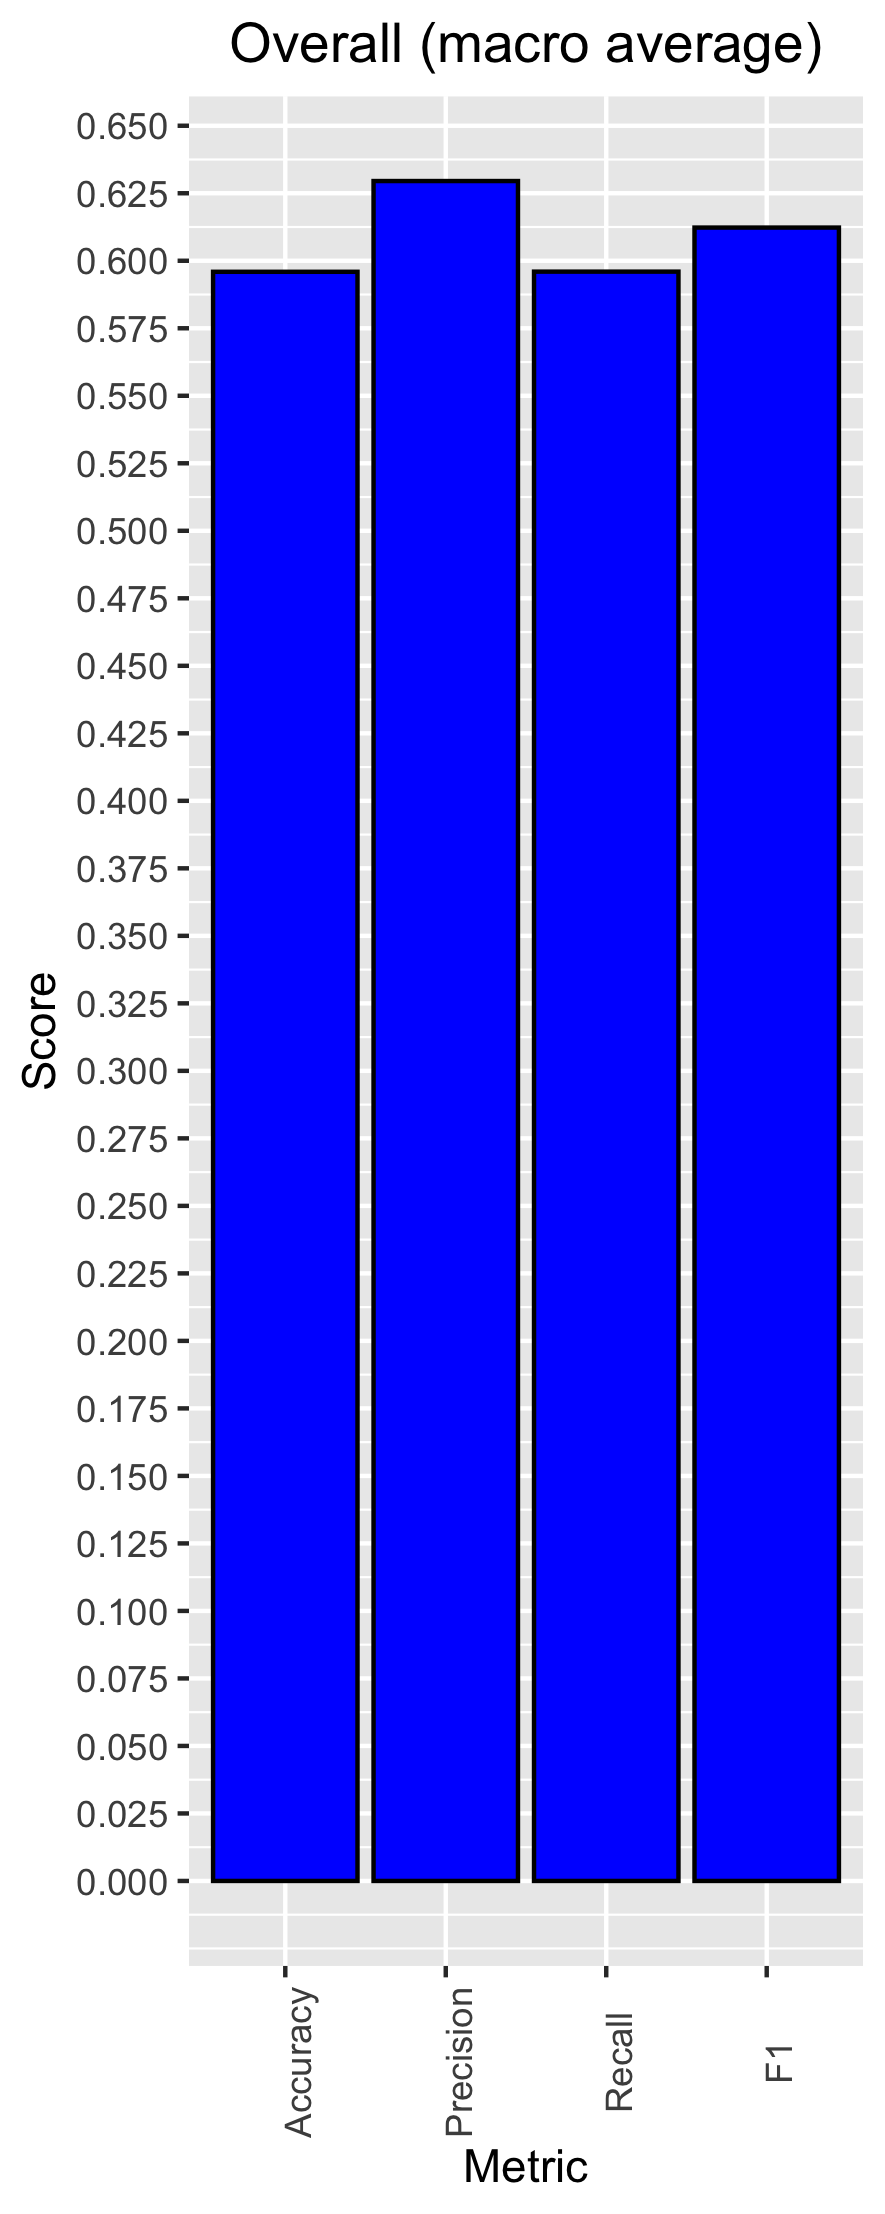
\includegraphics[width=4.25cm]{../images/rpart_performance.png}
		\caption{Decision tree.}
	\end{subfigure}
	\caption{Performance dei modelli (macro average).}
\end{figure}


\begin{table}[H]
	\begin{center}
		\begin{tabular}{ | l | c | c | c | c |  c | c |}
			\hline
			& \textbf{Precision+} & \textbf{Recall+} &\textbf{ F1+ }	& \textbf{Precision-} &\textbf{ Recall-} & \textbf{F1-} \\
			\hline
			\textbf{SVM - RBF} & 0.59860 & 0.67530  & 0.63313 &
												    0.63433 & 0.55098 & 0.58766\\
			\textbf{SVM - Linear} & 0.59600 & 0.73135 & 0.65625&
													0.65406 & 0.50413 & 0.56872\\
			\textbf{Decision tree} & 0.56467&  0.84469 & 0.67633 & 
										0.69437 & 0.34724 & 0.45957 \\
			\hline
		\end{tabular}
	\end{center}
	\caption{Confronto performance dei modelli distinguendo tra classe positiva e negativa.}
\end{table}




\begin{table}[H]
	\begin{center}
		\begin{tabular}{ | l | c | c | c | c |  c |}
			\hline
			& \textbf{Accuracy} & \textbf{Precision} &\textbf{ Recall }	& \textbf{F1} &\textbf{ AUC} \\
			\hline
			\textbf{SVM - RBF} & 0.61309 & 0.61640 & 0.61139  & 0.61800 & \textbf{0.66106} \\
			\textbf{SVM - Linear} & 0.61771 & 0.62503 & 0.61774 & 0.62136 & 0.65601 \\
			\textbf{Decision tree} & 0.59592 & 0.62921 & 0.59571 	& 0.61285 & 0.59734\\
			\hline
		\end{tabular}
	\end{center}
	\caption{Confronto performance dei modelli (macro average).}
\end{table}


\section{Modelli a confronto}
Sono stati messi a confronto i modelli di decision tree, di svm
allenata con kernel radiale e una svm allenata con kernel lineare.

\subsection{Confronto secondo metrica ROC}

\begin{figure}[H]
	\centering
	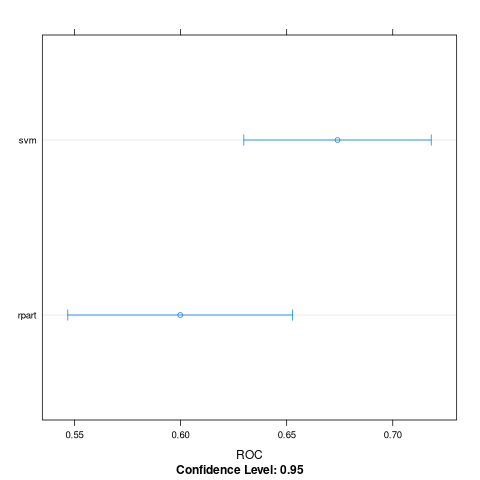
\includegraphics[width=13cm]{../images/compare_dot_plot.png}
	\caption{Dotplot per metrica ROC.}
	\label{fig:compare_dot_plot}
\end{figure}

\begin{figure}[H]
	\centering
	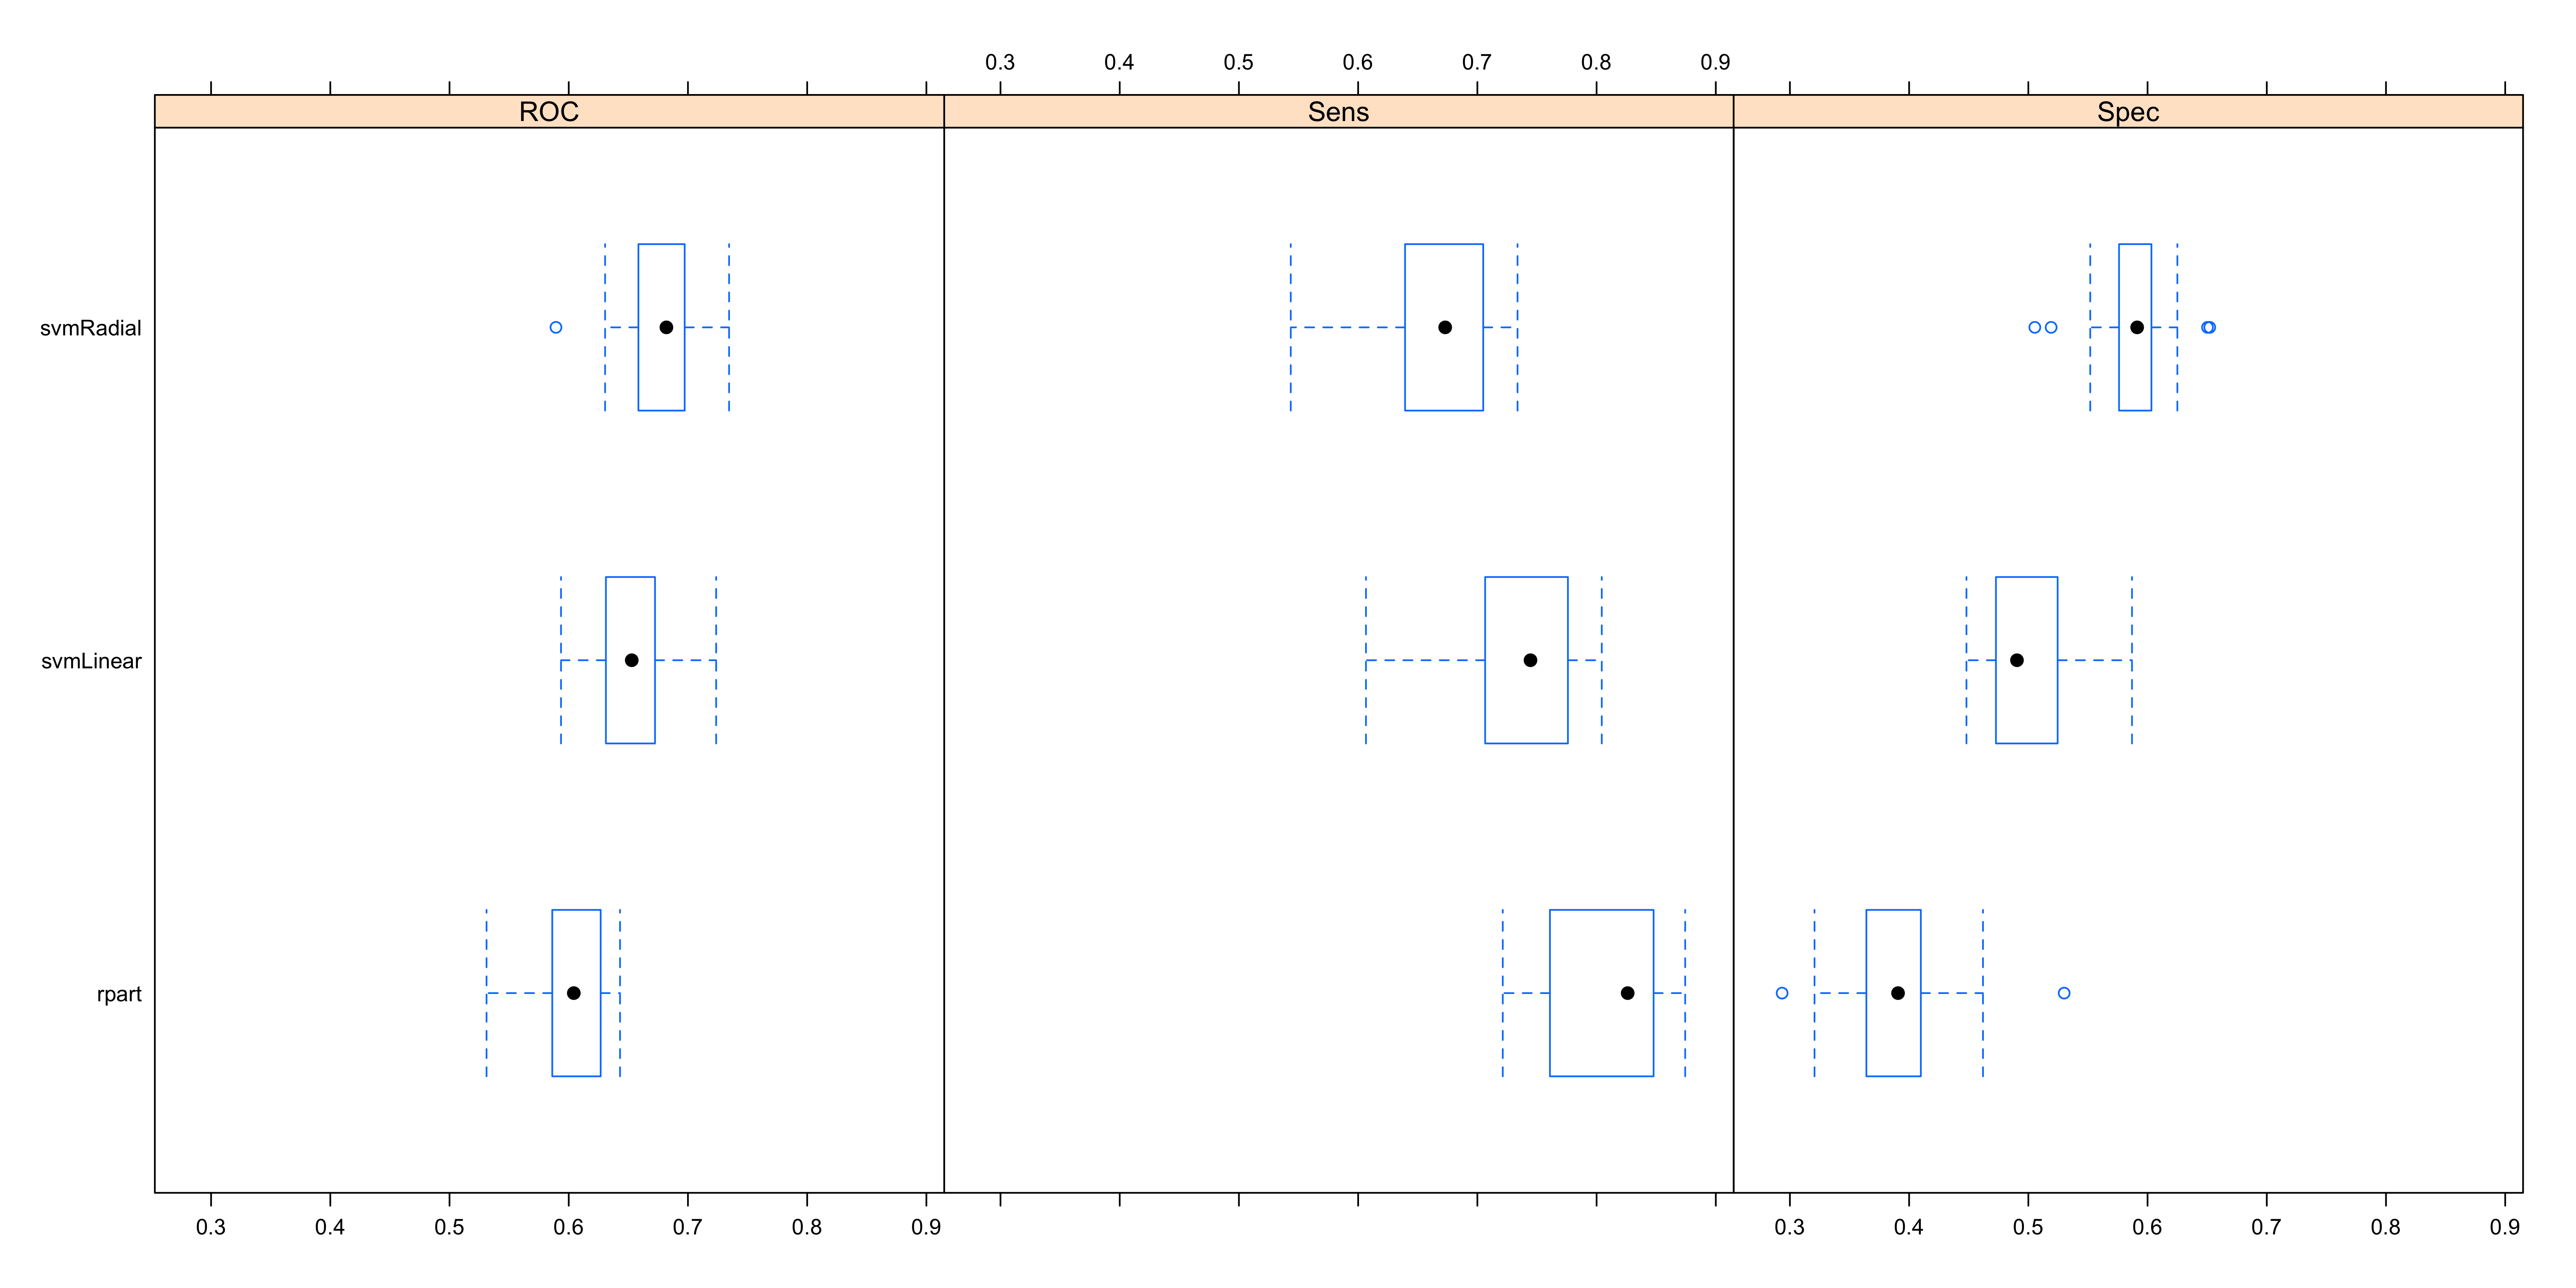
\includegraphics[width=13cm]{../images/compare_bw_plot.png}
	\caption{Dotplot per metrica ROC.}
	\label{fig:compare_bw_plot}
\end{figure}

\begin{figure}[H]
	\centering
	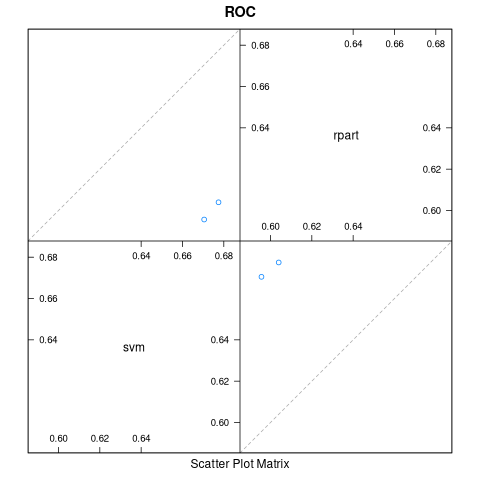
\includegraphics[width=13cm]{../images/compare_splom_plot.png}
	\caption{Scatter plot per metrica ROC.}
	\label{fig:compare_splom_plot}
\end{figure}

\subsection{Confronto Timings} Il modello support vector machine
risulta più lento per quanto riguarda i tempi di training, soprattuto se viene utilizzato il kernel radial basis function. Decision tree è quello più veloce.

\begin{table}[H]
	\begin{center}
		\begin{tabular}{ | l | c | c |}
			\hline
			& \textbf{Everything} & \textbf{Final model} \\
			\hline
			\textbf{SVM - RBF kernel} & 1286.484  & 43.524 \\
			\textbf{SVM - Linear kernel} & 666.136 & 34.730 \\
			\textbf{Decision tree} & 16.049 & 0.884  \\
			\hline
		\end{tabular}
	\end{center}
	\caption{Tempi per il training dei modelli.}
\end{table}

I tempi di training in tabella sono espressi in secondi. La colonna Everything si riferisce al training con la tecnica 10-fold cross validation mentre final model indica il training del modello utilizzando tutto il dataset. Per la fase di training vengono sfruttati più cores in modo tale da ridurre i tempi di training.